\documentclass[tikz,border=10pt]{standalone}
\usepackage{amsmath}
\usepackage{amssymb}
\usepackage{tikz}
\usetikzlibrary{arrows.meta,calc}

\definecolor{figazul}{RGB}{2,132,199}
\definecolor{figrojo}{RGB}{220,38,38}
\definecolor{figverde}{RGB}{22,163,74}

\begin{document}
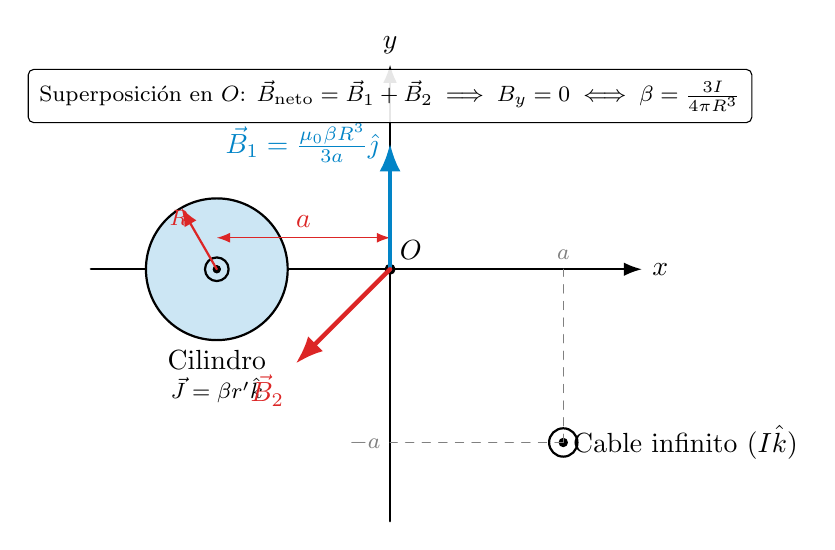
\begin{tikzpicture}[>=Latex, line cap=round, line join=round]
  % Ejes cartesianos
  \draw[->, thick] (-3.8,0) -- (3.2,0) node[right] {$x$};
  \draw[->, thick] (0,-3.2) -- (0,2.6) node[above] {$y$};
  \node[above right] at (0,0) {$O$};
  \fill (0,0) circle (2pt);

  % Escala: a = 2.2 cm
  % 1. Cilindro macizo centrado en r1 = -a*i = (-2.2, 0), radio R = 0.9 < a
  \coordinate (Cil) at (-2.2, 0);
  \draw[thick, fill=figazul!20] (Cil) circle (0.9);
  \fill[color=black] (Cil) circle (1.5pt);
  \node[below] at (-2.2, -0.9) {Cilindro};
  \node[below, font=\footnotesize] at (-2.2, -1.25) {$\vec{J} = \beta r'\hat{k}$};

  % Símbolo de corriente saliente en el cilindro
  \draw[thick] (Cil) circle (0.15);
  \fill (Cil) circle (0.05);

  % Cota del radio R del cilindro
  \draw[->, thick, color=figrojo] (Cil) -- ++(120:0.9);
  \node[above left, color=figrojo, font=\footnotesize] at ($(Cil) + (120:0.5)$) {$R$};

  % Cota de distancia a desde el origen
  \draw[<->, thin, color=figrojo] (-2.2, 0.4) -- (0, 0.4) node[midway, above, color=figrojo] {$a$};

  % 2. Cable infinito en r2 = a(i - j) = (2.2, -2.2)
  \coordinate (Cable) at (2.2, -2.2);
  \draw[thick] (Cable) circle (0.18);
  \fill (Cable) circle (0.06);
  \node[right] at (Cable) {Cable infinito ($I\hat{k}$)};

  % Líneas de proyección del cable hacia ejes
  \draw[dashed, thin, color=gray] (Cable) -- (2.2, 0) node[above, font=\footnotesize] {$a$};
  \draw[dashed, thin, color=gray] (Cable) -- (0, -2.2) node[left, font=\footnotesize] {$-a$};

  % Vectores de campo en el origen O
  % B1 debido al cilindro en (-a, 0): corriente +z -> regla mano derecha -> B1 apunta en +y
  \draw[->, ultra thick, color=figazul] (0,0) -- (0, 1.6) node[left, color=figazul] {$\vec{B}_1 = \frac{\mu_0\beta R^3}{3a}\hat{\jmath}$};

  % B2 debido al cable en (a, -a): vector desde cable a O es (-a, a).
  % r_obs = (-i + j)/sqrt(2). B2 = z_hat x r_obs = (-j - i)/sqrt(2) = en dirección -i - j
  \draw[->, ultra thick, color=figrojo] (0,0) -- (-1.2, -1.2) node[below left, color=figrojo] {$\vec{B}_2$};

  % Componentes y condición By = 0
  \node[draw, rounded corners=2pt, inner sep=4pt, fill=white, fill opacity=0.9, text opacity=1, font=\footnotesize] at (0, 2.2)
    {Superposición en $O$: $\vec{B}_{\text{neto}} = \vec{B}_1 + \vec{B}_2 \implies B_y = 0 \iff \beta = \frac{3I}{4\pi R^3}$};
\end{tikzpicture}
\end{document}
